\documentclass{beamer}
\usepackage{HECbeamer}
\usepackage{icomma}

\title[\color{white}{MATH 60604 \S~5b - Exemple de données longitudinales}]{\texorpdfstring{MATH 60604 \\Modélisation statistique \\ \S~5b - Exemple de données longitudinales}{MATH 60604 \\Modélisation statistique \\ \S~5b - Exemple de données longitudinales}}
\author{}
\institute{HEC Montréal\\
Département de sciences de la décision}
\date{} 

\begin{document}
\frame{\titlepage}

\begin{frame}
\frametitle{Exemple: évolution dans le temps du désir de vengeance}
\bi
\item Cet exemple traite du phénomène de vengeance des consommateurs qui est en forte croissance avec les possibilités qu'offre internet. 
\item Nous nous limiterons à étudier l'impact de certaines variables sur le désir de vengeance et aussi de voir comment le désir de vengeance évolue dans le temps. 

\item Les données utilisées ici sont fictives mais dans l'étude, elles provenaient de personnes qui s'étaient plaintes d'une firme sur les sites \code{ConsumerAffairs.com} et \code{RipOffReport.com}.
\item Cinq vagues de questionnaires ont été envoyés à ces personnes, à des intervalles de deux semaines.
\ei
\end{frame}

\begin{frame}
\frametitle{Exemple: évolution dans le temps du désir de vengeance }
\bi
\item \textbf{Variable dépendante d'intérêt}: le désir de vengeance, mesuré dans chaque questionnaire. 
\bi

\item Moyenne de cinq items sur une échelle de Likert allant de pas du tout d'accord (\texttt{1}) à tout à fait d'accord (\texttt{7}). 
\item Par exemple, l'un des items est « Je voulais prendre des mesures pour causer des problèmes à l'entreprise ».
\ei
\item \textbf{Variables explicatives}: seulement mesurées lors de la première vague --- le sexe, l'âge et deux variables mesurant des comportements de vengeance :
\bi
\item \textbf{plainte vindicative}, basée sur des items tel que « je me suis plaint des services de l'entreprise pour faire passer des moments difficiles au service à la clientèle ».
\item \textbf{bouche-à-oreille négatif}, basée sur trois items tel que « j'ai colporté des commentaires négatifs sur l'entreprise par bouche-à-oreille ».
\ei
\ei
\end{frame}

\begin{frame}
\frametitle{Données \texttt{vengeance}}
\bi
\item Un échantillon de 80 personnes ont participé à l'étude. 
\item Les données sont dans le fichier \code{vengeance.sas7bdat}. 
\item Les variables sont 
\bi

\item {\code{id}}: identification de la personne (entier allant de 1 à 80).
\item {\code{t}}: temps de mesure (1 à 5).
\item {\code{vengeance}}: désir de vengeance (variable dépendante).
\item {\code{sexe}}: homme (\texttt{0}) ou femme (\texttt{1}).
\item {\code{age}}: âge (en années).
\item {\code{vc}}: score pour items liées aux plaintes vindicatives
\item {\code{wom}}: score pour items liés au bouche-à-oreille négatif.
\ei
\ei
\end{frame}

\begin{frame}[fragile]
\frametitle{Données des trois premiers individus}
\begin{tcolorbox}[colback=white, colframe=hecblue, title=Code \SASlang{} pour imprimer un sous-ensemble des données]
\begin{verbatim}
proc print data=modstat.vengeance(where=(id<4)); 
run;
\end{verbatim}
\end{tcolorbox}
\begin{center}
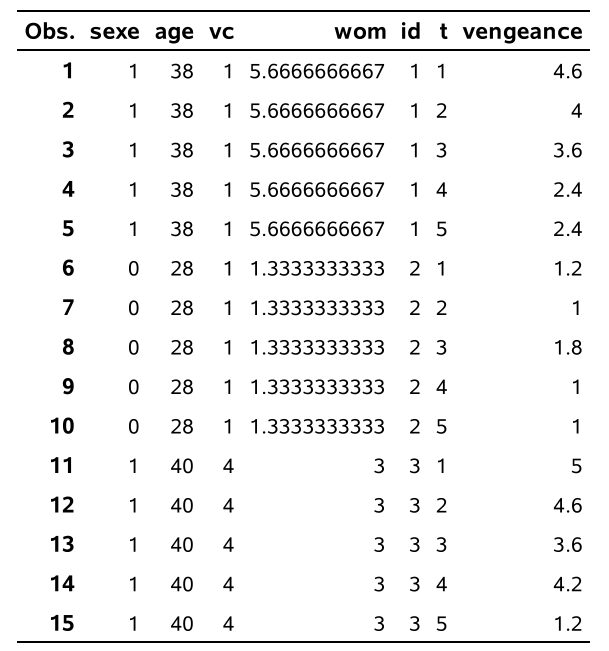
\includegraphics[width = 0.5\linewidth]{img/c5/diapos6-e01}
\end{center}

\end{frame}

\begin{frame}
\frametitle{Évolution dans le temps du désir de vengeance}
\bi
\item Il est important de comprendre la \alert{structure} des données, ici une ligne par observation. 
\item Dans le fichier, on a cinq lignes par personne: 
\bi
\item  aucune valeur manquante, 
\item chacune des cinq lignes correspond à un temps de mesure \code{t}. 
\ei
\item La seule variable qui évolue est \code{vengeance}.
\bi
\item Les variables \code{sexe}, \code{age}, \code{vc} et \code{wom} ont seulement été mesurées au temps \texttt{t=1}, elles sont reportées pour chaque temps de mesure. 
\ei
\item Lorsqu'on a des modèles longitudinaux, il est souvent nécessaire de formater les données pour avoir une ligne par mesure (format long).
\ei
\end{frame}



\begin{frame}[fragile]
\frametitle{Statistiques descriptives avec données répétées}
 Il faut être prudent si on calcule des statistiques descriptives pour les variables qui sont fixes, comme \code{sexe}, \code{age}, \code{vc} et \code{wom}. 
\bi 
\item La moyenne empirique sera identique uniquement parce qu'on a pas le même nombre d'observations par personne, $T=5$.
\item L'estimée de l'erreur-type de la moyenne sera trop petite parce que le nombre réel de mesures uniques $N=80$ n'est pas égale au nombre de lignes de la base de données $NT=400$.
\ei
\end{frame}
\begin{frame}
\frametitle{Exemple de calcul}
L'âge moyen des $N=80$ participants est $\overline{\code{age}}= 42.075$ ans.
\bi
\item l'écart-type est $S=7.49$ et $\mathsf{se}(\overline{\code{age}})= 0.837$, où
\[S^2=\frac{\sum_{i=1}^N (\code{age}_i-\overline{\code{age}})^2}{N-1}, \qquad \mathsf{se}(\overline{\code{age}})=\frac{S}{\sqrt{80}}.\]
\ei
Comparez avec le calcul suivant \textbf{qui n'est pas correct}.
\[S^2_{*} = \frac{\sum_{i=1}^{NT} (\code{age}_i-\overline{\code{age}})^2}{(NT-1)} \approx S^2, \qquad \mathsf{se}(\overline{\code{age}}) \neq\frac{S_*}{\sqrt{400}} = 0.37 \]
\end{frame}

\begin{frame}[fragile]
\frametitle{Statistiques descriptives avec SAS}
On peut par contre se limiter aux mesures pour un instant donné.
\begin{tcolorbox}[colback=white, colframe=hecblue, title=Code SAS pour calculer les statistiques descriptives]
\begin{verbatim}
proc means data=modstat.vengeance(where=(t=1)); 
var sexe age vc wom; 
run; 
proc corr data=modstat.vengeance(where=(t=1)); 
var sexe age vc wom; 
run;
\end{verbatim}
\end{tcolorbox}

\end{frame}

% \begin{frame}[fragile]
% \frametitle{Statistiques descriptives pour le désir de vengeance}
% \bi
% \item Nous avons regardé les statistiques descriptives de quatre variables explicatives mais il y en a également une cinquième.
% \bi \item la variable temps, $\code{t}\in \{1, 2, 3, 4, 5\}$.
% \ei
% \item On peut en effet penser que le désir de vengeance augmente (ou diminue) au fur et à mesure que le temps passe. 
% \ei 
% \end{frame}
\begin{frame}[fragile]
\frametitle{Visualisation de l'effet temporel}
\bi \item 
 Il est plausible que le désir de vengeance varie en fonction du temps. 
 \item Une façon simple de visualiser l'évolution du désir de vengeance est de tracer un graphique de \code{vengeance} en fonction de $t$ \alert{pour chaque personne}.
\ei
\begin{tcolorbox}[colback=white, colframe=hecblue, title=Code \SASlang{} pour dessiner un graphique spaghetti]
\begin{verbatim}
proc sgplot data=modstat.vengeance;
series x=t y=vengeance / group=id;
run;
\end{verbatim}
\end{tcolorbox}

\end{frame}




\begin{frame}[fragile]
\frametitle{Graphique spaghetti}
\begin{center}
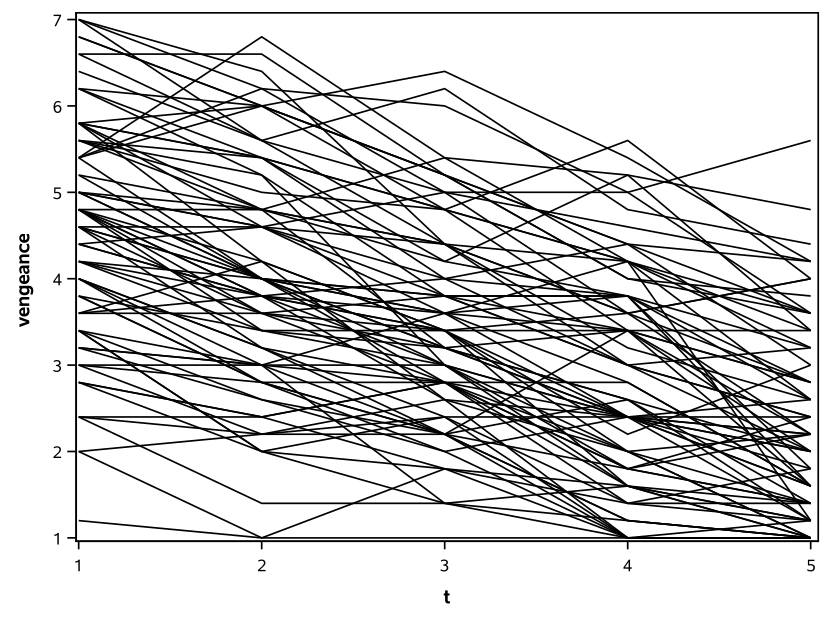
\includegraphics[width = 0.7\linewidth]{img/c5/diapos6-e02}
\end{center}
Ce graphe contient 80 courbes (une par personne) qui s'entrecroisent. Bien que difficile à interpréter, on peut déceler une
tendance: en moyenne, la valeur du désir de vengeance tend à décroître au fil du temps.
\end{frame}
\end{document}
